%!TEX encoding = UTF-8 Unicode
% -*- coding: UTF-8; -*-
% vim: set fenc-utf-8

\chapter{Maquette des interfaces}
\label{s:maquettes_interfaces}

Ce chapitre présente les maquettes des principales interfaces de l'application VisuaLigue.
Une courte explication des fonctionnalités moins évidentes est également présente à la suite des figures si nécessaire.

\begin{figure}[htpb]
    \centering
    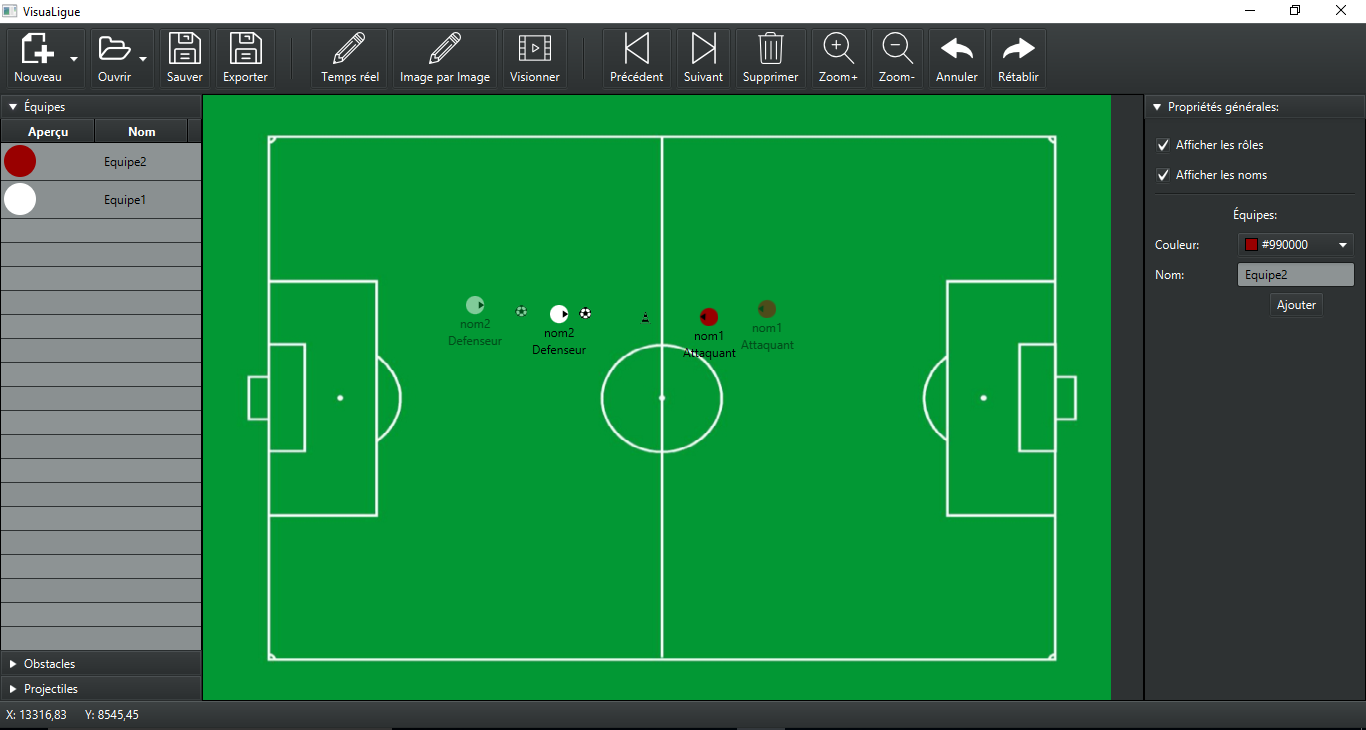
\includegraphics[scale=0.6]{fig/gui/creationStackPane.png}
    \caption{Interface pour la création des stratégies}
    \label{fig:gui:creationStackPane}
\end{figure}

L'interface \ref{fig:gui:creationStackPane} permet l'édition des stratégies, soit en mode image par image ou en mode temps réel.
Elle apparait lorsque l'on appuie sur le bouton temps réel ou image par image.
Un menu à gauche permet de glisser des joueurs, obstacles ou projectiles sur le terrain.
Un menu à droite permet d'ajouter une équipe dans la liste des joueurs à gauche.
Il permet aussi de choisir si on affiche le rôle et le nom des joueurs sur le terrain.
Si on clique sur un joueur sur le terrain, le menu à droite change pour éditer son nom, son rôle et son orientation et une case est présente pour décider si le joueur possède le projectile.
Les icônes "suivant" et "précédent" permettent respectivement d'avancer ou de reculer d'une image dans le mode image par image.
Les étiquettes "x" et "y" dans le bas de la fenêtre correspondent aux coordonnées de la souris sur le terrain en unités réelles.
La transparence de certains joueurs sur la figure ci-dessus correspond à des éléments qui proviennent d'une image précédente lors de l'édition en mode image par image.
Le groupe de boutons en haut à droite permet d'effectuer diverses actions par rapport à l'édition de la stratégie.
Le groupe du milieu permet de changer le mode.
Le groupe de gauche permet des actions plus générales.

\begin{figure}[htpb]
    \centering
    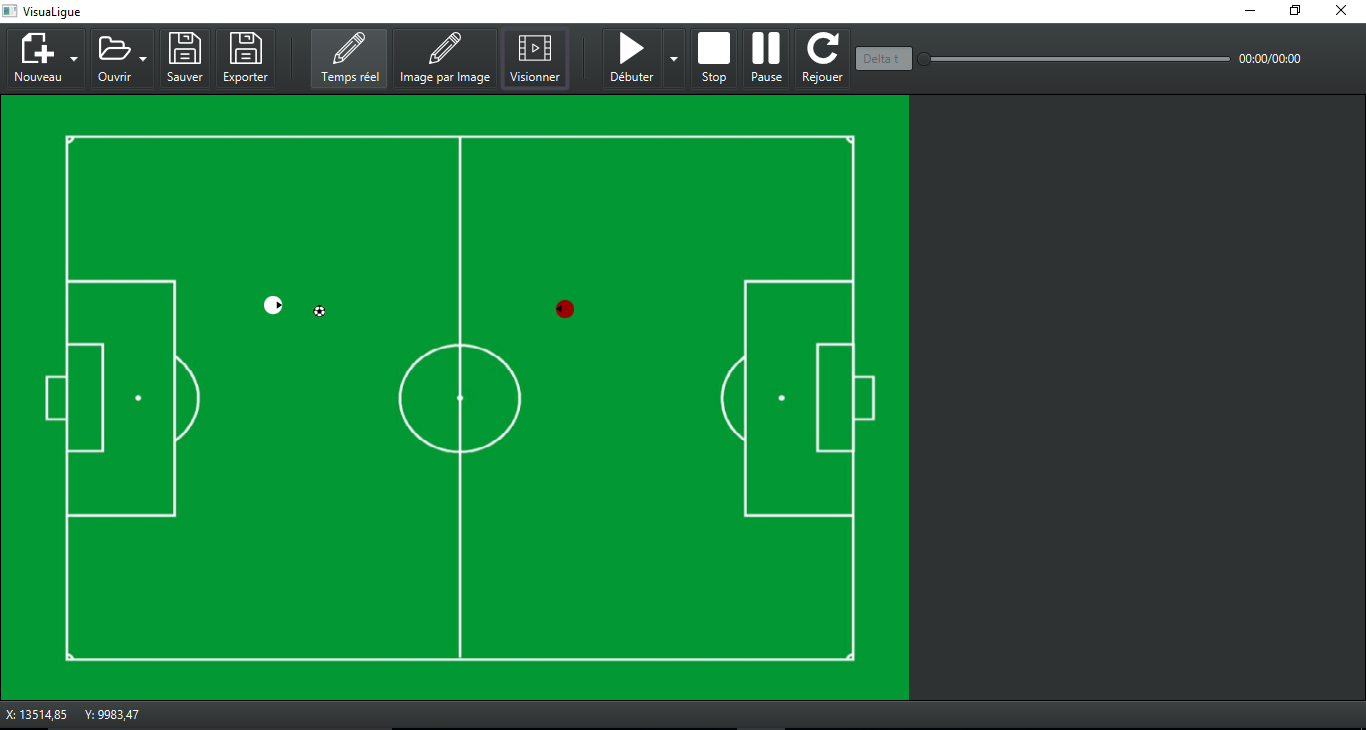
\includegraphics[scale=0.6]{fig/gui/mediaContent.png}
    \caption{Interface pour la visualisation des stratégies}
    \label{fig:gui:mediaContent}
\end{figure}

L'interface \ref{fig:gui:mediaContent} permet la visualisation des stratégies préalablement créées.
Elle apparait lorsque l'on appuie sur le bouton visionner.
En plus des boutons habituels de visionnement de vidéos, on y retrouve un curseur glissant permettant de se déplacer facilement à n'importe quel temps de la stratégie.
Il y a aussi une boîte de saisie et un bouton associé pour rejouer une séquence de la stratégie.
Les coordonnées de la souris sont encore affichées.

\begin{figure}[htpb]
    \centering
    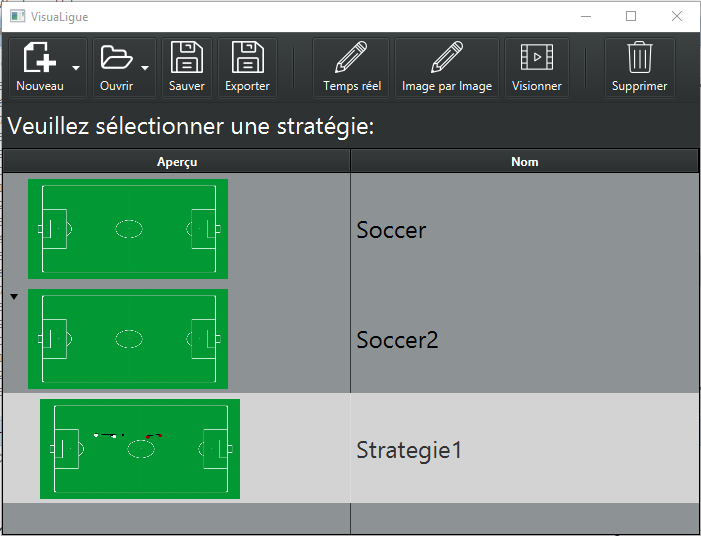
\includegraphics[scale=0.6]{fig/gui/openStrategy.png}
    \caption{Interface de gestion des stratégies et des sports}
    \label{fig:gui:openStrategy}
\end{figure}

L'interface \ref{fig:gui:openStrategy} permet la gestion des stratégies et des sports.
Après avoir sélectionné une stratégie ou un sport, une multitude de choix s'offre à l'entraîneur.
Il peut supprimer un sport ou une stratégie, visionner une stratégie, ou bien l'éditer soit en mode temps réel ou en mode image par image.
\newpage

\begin{figure}[htpb]
    \centering
    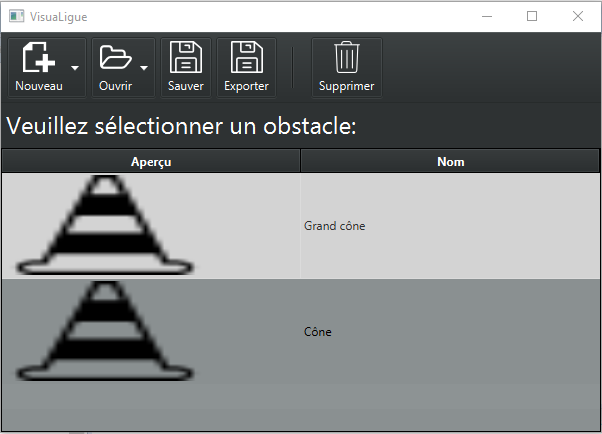
\includegraphics[scale=0.6]{fig/gui/openObstacle.png}
    \caption{Interface de gestion des obstacles}
    \label{fig:gui:openObstacle}
\end{figure}

L'interface \ref{fig:gui:openObstacle} permet la gestion des obstacles.
On peut visualiser les types d'obstacles et en supprimer via cette interface.

\newpage

\begin{figure}[htpb]
    \centering
    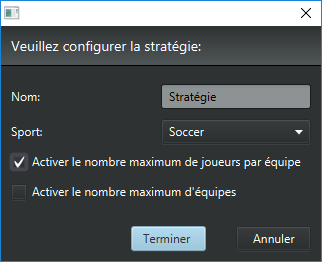
\includegraphics[scale=0.6]{fig/gui/newStrategy.png}
    \caption{Interface de création des stratégies}
    \label{fig:gui:newStrategy}
\end{figure}

La fenêtre de dialogue \ref{fig:gui:newStrategy} permet de créer une stratégie.
Elle apparaît lorsque l'on appuie sur le bouton nouveau/stratégie.
Tous les paramètres nécessaires à la création d'une stratégie y sont présents.

\begin{figure}[htpb]
    \centering
    \includegraphics[scale=0.6]{fig/gui/newSport.png}
    \caption{Interface de création des sports}
    \label{fig:gui:newSport}
\end{figure}

La fenêtre de dialogue \ref{fig:gui:newSport} permet de créer un sport.
Elle apparaît lorsque l'on appuie sur le bouton nouveau/sport.
Tous les paramètres nécessaires à la création d'une stratégie y sont présents, y compris la configuration du terrain, du projectile et des rôles.

\newpage

\begin{figure}[htpb]
    \centering
    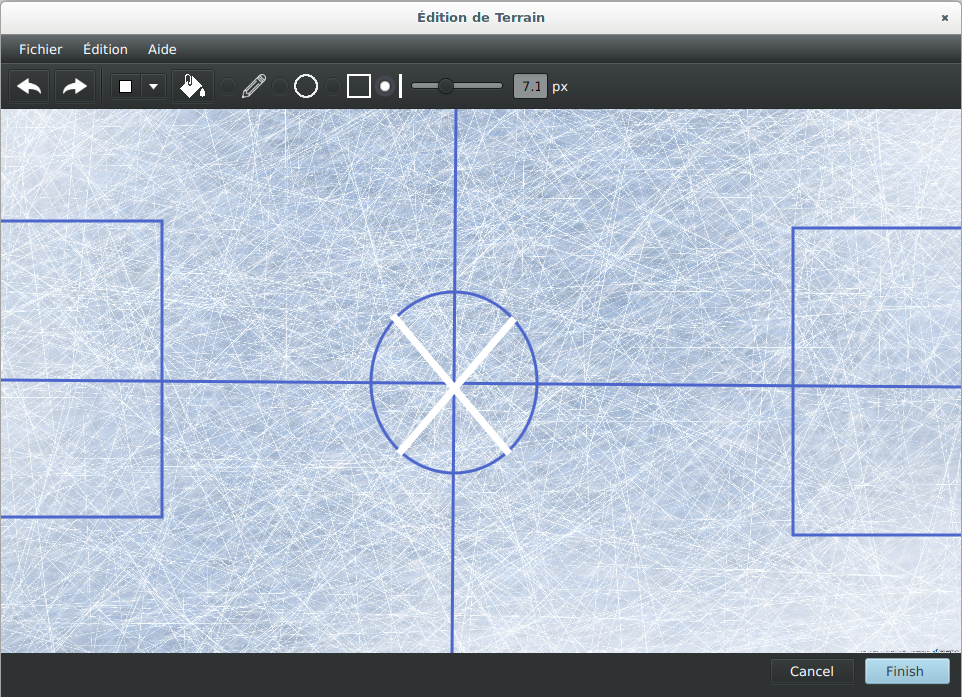
\includegraphics[scale=0.35]{fig/gui/gui_edit_field.png}
    \caption{Interface d'édition de terrain}
    \label{fig:gui:terrain}
\end{figure}

La fenêtre de dialogue \ref{fig:gui:terrain} permet de créer une image de terrain.
Elle apparaît lorsque l'on appuie sur le bouton dessiner dans le dialogue de création de sports.

\begin{figure}[htpb]
    \centering
    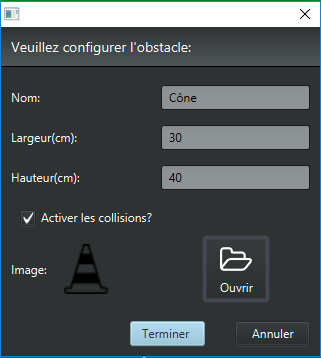
\includegraphics[scale=0.6]{fig/gui/newObstacle.png}
    \caption{Interface de création des obstacles}
    \label{fig:gui:newObstacle}
\end{figure}

La fenêtre de dialogue \ref{fig:gui:newObstacle} permet de créer un sport.
Elle apparaît lorsque l'on appuie sur le bouton nouveau/obstacle.
Tous les paramètres nécessaires à la création d'un obstacle y sont présents, y compris un champs pour activer les collisions ou non sur l'obstacle.

\newpage
